\chapter{Preliminary studies} % What is lean saying about this
\label{chap:PreliminaryStudies}
This chapter presents the preliminary studies done in the project. It sums up all research conducted throughout the project lifetime. Because of the \gls{LSU}, the research was not done before the team began the project. Research regarding a specific topic was done before it was needed. The chapter also includes studies on existing and similar systems, software development models and technical requirements. 

\section{Existing system}
The customer representative had already made a simple prototype of the application. This prototype was never shown to the development team as he did not want it to affect the final product. In addition, he wanted to see how the result would be when developed using \gls{LSU}.  
\section{Similar systems}
There exists many similar applications where the user can scan barcodes, get book information from an information provider like Google Books and have a library on their phone. The main difference from many of those applications and the system created during this project, is the possibility to share books. Some applications had the possibility to add borrowers to books, but only with a tag that could only be updated locally. The two most similar systems that were found was BookCrossing and BookBuddy.

BookCrossing is a webpage for sharing books.\cite{book-crossing} The concept is simply that people can share books by giving it to a friend, or just leaving them in public places where other readers can find it and read it. When this reader is done with the book he can give it to one of his friends or leave it in another public place for someone else to find. When a person picks up a book he is supposed to leave a brief note so that others will know what has happened to the book. This way the person who registered the book, and other users, can follow how the book is travelling around the world. To register a book, the book is labeled with a BookCrossingID, BCID, which is the identification used to add notes to the book and follow the books travel.

A difference between BookCrossing and the system created during this project, is that BookCrossing uses a webpage and not a mobile application. This means that BookCrossing demands more effort to add a book then the application of this project. Since the book can not be scanned it must be added manually. In addition a label must be made and added to the book. Another different is that BookCrossing mainly share books to stranger, while the application explained in this report is made for mainly sharing books with acquaintances, and that you expect to get the book back someday. 

BookBuddy is an iOS application which allows you to quickly find any book in your library, share your favorite books, and keep track of borrowed and lent books.\cite{book-buddy} BookBuddy pro cost \$4.99, but they also have a free version which was the one considered as a potential competitor to the application explained in this report. The free version is only local, which means that when a user adds a borrower to one of its books it was only visible on the user's phone, and could not be seen from the phone of the borrower. In addition did BookBuddy not give the user the possibility of viewing other users' library.

\section{Software development models}
Selection of software development model is a crucial part of the development process because the model set certain standards to how a project will be conducted. This section describes possible development methodologies and concludes with what was used in this project. 

\subsection{The Waterfall Model}
The waterfall model is a sequential development process where every step of the process has to be followed in the decided sequence.\cite[p.~30-32]{software-engineering} This model can be useful if you know what you are going to make and how you are going to make it. This was not the case in this project. Because the product described in this report is supposed to be able to be used by many users, it is important to make it after the users wish. Since the development team do not know exactly what the users want, they will be dependent on feedback, which again most likely will mean changes. Therefore an agile software development would be better.

\subsection{Scrum}
Scrum is an agile software development process that is based on the process being iterative and incremental.\cite{scrum} This development methodology is practical when knowing what the product will be, but not the technologies that will be used.

\subsection{Kanban}
Kanban is a method for managing knowledge work, that has been used for software development processes in later years. The point of Kanban in the context of software development is that team members pluck items of the \gls{backlog} when they are done with an item. The product owner can restructure the \gls{backlog} at any time, without disrupting the team. At project start up the team sets limit on the number of tasks that can be in the different parts of the process, for example in development and in testing. If a task 'A' is about to be sent to testing, but the amount of tasks in testing is at its limit, then the developer moves to do testing until the number of tasks there has gone down. Then task 'A' is moved to testing. This means that the team is collectively responsible for every part of the development process. \cite{kanban-intro} 

\subsection{The Lean startup} 
\label{lean-description}
The \gls{LSU} development methodology was created by Eric Ries in 2011.\cite{lean-startup} The goal of this process is to shorten the time of developing a product to be able to spend a minimal amount of resources to learn if you made something good or not. The \gls{LSU} methodology is based on not knowing what you are going to make, and not how you are going to make it. Key concepts of the \gls{LSU} are described here.

First there is the \gls{MVP}. The \gls{MVP} is “that version of the product that enables a full turn of the Build-Measure-Learn loop with a minimum amount of effort and the least amount of development time”.\cite[p.~72]{lean-startup} This product may have many lacks and bugs, but as long as it can provide validated learning, it is good enough.

Then comes the validated learning, which is everything that can be learned about the use of the application, or the users' needs. The principle is that the developers have to learn what the user really wants, not what they think they want.

Another concept is the build-measure-learn loop which describes a \gls{LSU} iterations and is at the core of the \gls{LSU} model. An illustration of this loop is found in figure \ref{fig:build-measure-learn}. In the illustration the "Design"-box equals Build. 
The feedback loop starts with an assumption of what the users of the product needs. Based on this assumption ideas on how to learn the answer to that assumption are generated and a \gls{MVP} is built based on those ideas. This \gls{MVP} can be everything from a sketch to a paper prototype to a functioning product. The use or other metrics are then measured from the \gls{MVP}. The choice of metrics are important in the \gls{LSU} because the iteration is pointless if it does not give any answers. Finally validated learning is achieved when the assumption is either confirmed or discarded.
\begin{figure}
\centering
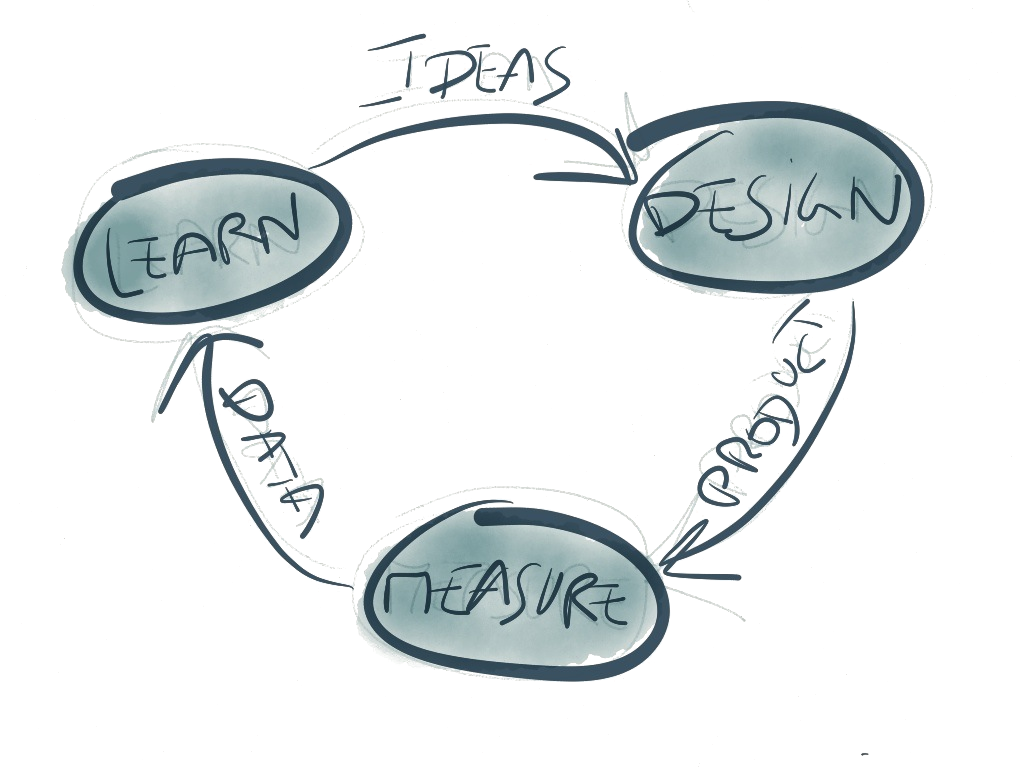
\includegraphics[height=6cm]{figs/build-measure-learn.png}
\caption{The Build-Measure-Learn feedback loop}
\label{fig:build-measure-learn}
\end{figure}

This cycle brings up the concept of pivot. What if no one will use your product? Or what if a new feature is unsuccessful? Then you have to pivot. That means scratch that idea and start from the beginning. If it is just a feature it is not a big problem, the feature will just be removed or kept without any improvements. However if it is the whole product the consequences are greater, but by using the \gls{LSU}s iterations this will probably not happen because it is confirmed on an early stage that at least some aspects of the product is desired by the user.  

\subsection{Conclusion}
In the first customer meeting where the team met the customer representative he explained why he wanted the product to be made using the \gls{LSU} methodology. As basis for his explanation he drew a two-dimensional grid shown in figure \ref{fig:lean-scrum-waterfall}. This illustration is also shown in figure \ref{fig:lean-scrum-waterfall2} where the illustration may be some what clearer.
He suggested that the team used lean because they do not know the marked of the product and as a consequence of that do not know what to develop. In accordance to the figure he drew that explained why the project should follow the \gls{LSU} methodology.

\begin{figure}
\centering
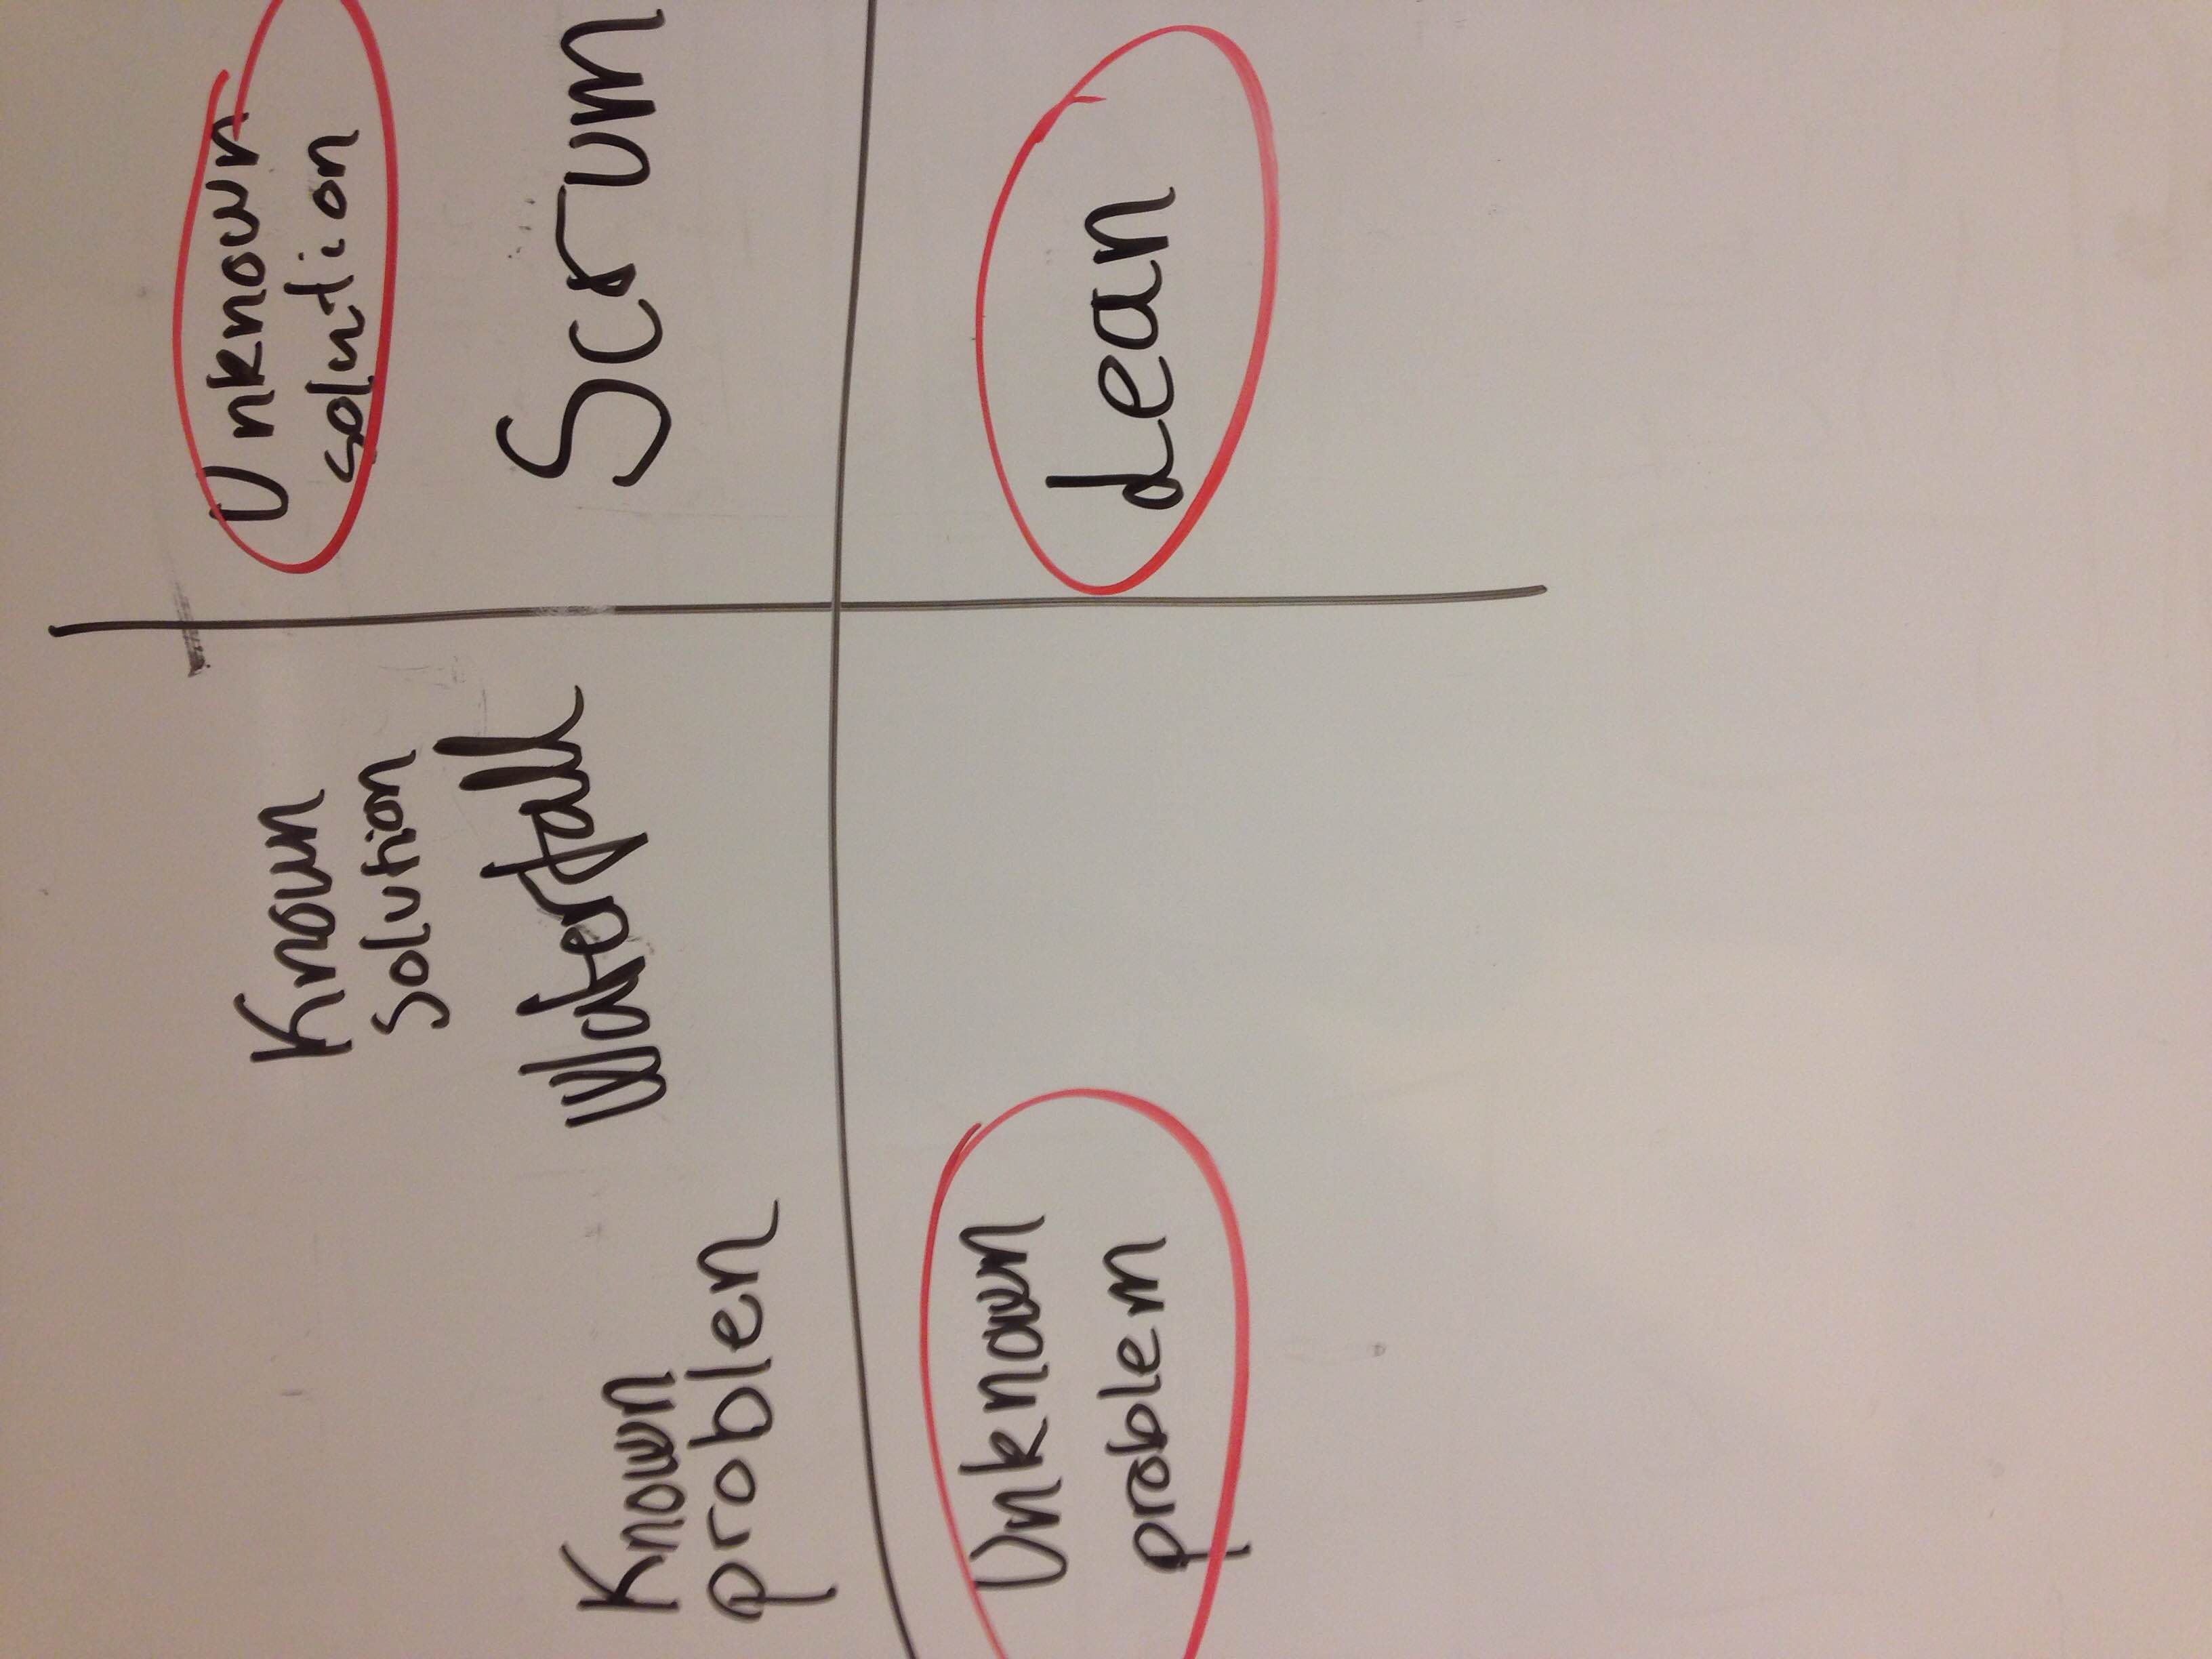
\includegraphics[height=6cm, angle =-90]{figs/lean-scrum-waterfall.JPG}
\caption{Figure drawn by the customer representative to explain the use of \gls{LSU}}
\label{fig:lean-scrum-waterfall}
\end{figure}

\begin{figure}
\centering
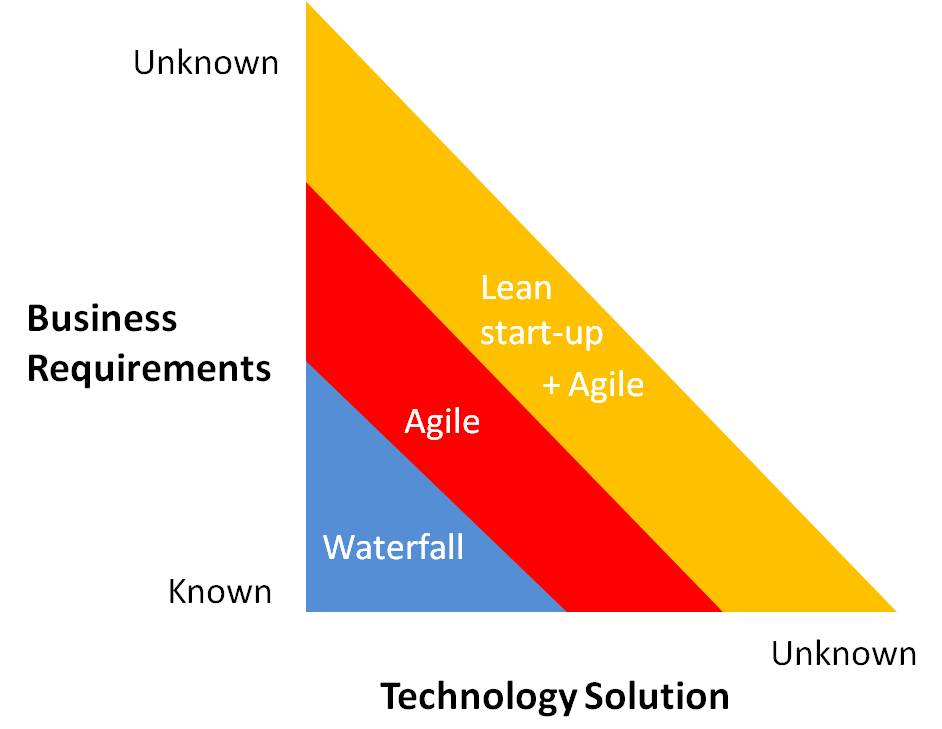
\includegraphics[height=7cm]{figs/lean-vs-other.jpg}
\caption{Illustration of the different areas where waterfall, agile methods and Lean Starup are best suited.}
\label{fig:lean-scrum-waterfall2}
\end{figure}

As mentioned the team will use The \gls{LSU} as development model for this project, but because it lacks a lot of structure the project's development process will be combined with some features from Scrum and kanban. The team will use a kanban board to keep track of the progress in the different versions.\cite[p. 137]{lean-startup} It will also be held daily stand-up meetings from scrum, and planning and retrospective meetings for each version.


\section{Technical studies}
This section describes the technical decisions and research that had to be made during this project.
\subsection{Information provider}
Because the product of this project is a book sharing system there is a need for an information provider to get information about the books. The team discussed and looked at some possibilities and ended up choosing Google Books as the initial information provider. The reason for this decision is that Google Books has a well documented API, and the service contains enough books for the initial use of the application.

\begin{table}[]
\centering
\begin{tabular}{|l|c|c|c|c|c|c|}
\hline
\textbf{Technologies} & \textbf{Stein-Otto} & \textbf{Øyvind} & \textbf{Markus} & \textbf{Torstein} & \textbf{Maren} & \textbf{Morten} \\ \hline
Java & x & x & x & x & x & x \\ \hline
Python & x & x & x & x & x & x \\ \hline
MySQL & x & x & x & x & x & x \\ \hline
HTML/CSS/JS & x & x & x &  & x &  \\ \hline
iOS & x & x & x &  & x &  \\ \hline
Android & x &  & x & x &  & x \\ \hline
AngularJS & x & x &  &  &  &  \\ \hline
Backend & x &  &  & x &  &  \\ \hline
Flask & x & x &  &  &  &  \\ \hline
libgdx & x &  &  & x &  &  \\ \hline
C\#, XAML &  &  & x &  &  &  \\ \hline
PHP & x &  & x &  &  &  \\ \hline
FXML &  &  &  &  & x &  \\ \hline
Jade &  & x &  &  &  &  \\ \hline
Firebase &  & x &  &  &  &  \\ \hline
NodeJS and expressjs. Sequelize & x &  &  &  &  &  \\ \hline
Webdev (Bower, Grunt, Gulp) & x &  &  &  &  &  \\ \hline
C &  &  &  &  &  & x \\ \hline
C++ &  &  &  &  &  & x \\ \hline
\end{tabular}
\caption{Technologies and platforms known prior to the project}
\label{table:prior-knowledge}
\end{table}

\subsection{Known technologies}
Table \ref{table:prior-knowledge} is a matrix of the different technologies that the team members have experience with, and this is also the background for the platforms and frameworks the team chose to work with.

\subsection{Android}
This section describes which tools, languages and libraries that were considered for making the Android application.

\subsubsection{Tools}
\begin{description}
    \item[Android Studio] \hfill \\
        Android Studio is an \gls{IDE} developed by Google. The \gls{IDE} is based on JetBrains' IntelliJ IDEA software and is specifically designed for development for the Android platform. Android Studios is a cross-platform IDE available on both Windows, Mac OS X and Linux, and offers tools such as a text editor, emulators and a compiler, making it a complete package for developing Android applications. In 2015 Google ended support for Android development in other applications, leaving Android Studio as the main tool for Android development.\cite{dead-eclipse}
    \item[Gradle] \hfill \\
        Gradle is a build automation tool integrated in Android Studio. Gradle automatically compresses all project source files from an Android Studio project into an Android application packages file, also knows as the .APK file. This .APK file can then be used to install the application on different devices. Gradle also handles the dependencies of the project. By specifying the necessary dependencies, external libraries are downloaded from the Maven repositories and included in the project.\cite{gradle}
\end{description}

\subsubsection{Languages}

There are some alternatives when developing applications for the Android operating system. However, Android supports only the Java programming language natively. Other options need to convert code in some way to support Android.

\begin{description}
    \item[Java] \hfill \\
        The Java programming language is the main language used for developing native applications for the mobile operating system Android. Java is one of the most common programming languages taught at \gls{NTNU}, and is therefore known prior to this project by every team member. 
    \item[HTML5, CSS and Javascript] \hfill \\
        An alternative to developing an native application for Android using the Java programming language is using a combination of HTML5, CSS and JavaScript for creating a cross-platform application. There exists tools which then translates code written in some language to the native language of a selected platform. 
    
    
    
\end{description}

Since every team member and especially the Android team knows Java prior to this project and that the customer wants applications developed native for each platform our decision of developing the Android application in Java was very easy. The main challenge of creating a native Android application is to learn how to write Java for the Android \gls{SDK}. 

\subsubsection{Libraries}

\begin{description}
    \item[Mixpanel] \hfill \\
        Mixpanel is an analytics service for analyzing how users use an application.\cite{mixpanel}
    \item[Otto event bus] \hfill \\
        Otto is a simple, light-weight event bus. Classes running on the main application thread can subscribe to the bus and listen to events, it is possible to publish events to the bus on any thread.\cite{otto}
    \item[Realm] \hfill \\
        Realm is a database solution for Android (Java) and iOS (Objective C and Swift).\cite{realm} It is a small, object oriented, and efficient database that enables storing data on the user's device, and sharing data safely among threads.
    \item[ZXing] \hfill \\
        ZXing ("zebra crossing") is an open-source barcode image processing library implemented in Java.\cite{zxing} ZXing is used for automatic recognizing of ISBN numbers from barcodes on books using the camera on an Android device.  
    \item[Google GSON] \hfill \\
        Google's GSON is a library for converting Java objects to and from JSON. Java objects can be serialized to the JSON-format, and likewise, deserialized from JSON to Java objects.\cite{gson}
\end{description}

\subsubsection{Conclusion}
It became natural to choose Java and Android studio as our main development platform for the Android application since our customer wanted a native application and the developers of the Android operating system, Google, suggests using Android studio. Since the team had little to no experience with Android development, the choice of different libraries to use is based on tips from the customer as well as choosing the first and best library that solves our problems. 

\subsection{iOS}
This section describes which tools, languages and libraries that were used to make the iOS application.

\subsubsection{Languages}
\begin{description}
    \item[Objective-C] \hfill \\
        Objective-C is the most used language when developing for Apple's platforms.\cite{programming-language-popularity-statistics} The language has evolved during the last 30 years, and is now offering a wide range of features and third party libraries. Although Objective-C is highly adaptable, it is evident that the syntax is outdated and more verbose than many modern languages. 
    \item[Swift] \hfill \\
        When Apple announced Swift in 2014, they presented it as the new preferred programming language for their platforms. It was more efficient than Objective-C and offered a simpler syntax.\cite{objc-swift-comparison} As the language is relatively new, it is still frequently updated. The syntax is still being updated, which may result in additional work when new versions are released.
    \item[Others] \hfill \\
        There are other languages such as Objective-C++ that can be used when developing applications for iOS, but due to limited experience using these languages in the team, they were not considered.
\end{description}

\subsubsection{Dependency managers}
For many years, CocoaPods was the obvious choice of dependency manager for iOS.\cite{cocoapods} A new project called Carthage was released in 2014, and has grown rapidly since then.\cite{carthage}

\begin{description} 
    \item[CocoaPods] \hfill \\
        Cocoapods is the most popular dependency manager for Objective-C and Swift. It offers thousands of libraries and makes adding dependencies, keeping them up to date, and scaling the project effortless. In addition to retrieving dependencies, it also integrates the dependencies into existing projects automatically. In most cases this makes working with external libraries easier, but it also induces an abstraction that is hard to debug if it breaks.
    \item[Carthage] \hfill \\
        Carthage's goal is to offer a new dependency manager that is smaller, easier to use, and simpler than CocoaPods. It will manage your dependencies, but not integrate them into the project automatically. An increasing number of third party libraries are available through Carthage.
\end{description}


\subsubsection{Development environment}
When developing native applications for Apple's platforms choosing development environment is a simple task.

\begin{description} 
    \item[Xcode] \hfill \\
        Xcode is Apple's proprietary integrated development environment and offers a complete package containing all necessary tools such as text editor, compilers, interface builder, and simulators.\cite{xcode} Xcode can also be used when preparing and uploading the application to AppStore for testing and distribution.
\end{description}


\subsubsection{Other libraries} 
\begin{description}
    \item[Realm] \hfill \\
        Realm is a database designed for mobile platforms.\cite{realm} It is a small, object oriented, and efficient database that enables storing data on the user's device, and sharing data safely among threads.
    \item[Alamofire] \hfill \\
        Alamofire is a small networking library which is easier to use than Apple's native NSURLSession.\cite{alamofire} The library exploits concepts from functional programming by allowing chaining of response handlers, and offers practical features such as automatic JSON serialization.\cite{json}
    \item[MTBBarcodeScanner] \hfill \\
        MTBBarcodeScanner offers a simplified \gls{API} for working with Apple's integrated barcode scanner functionality.\cite{mtbbarcodescanner}
\end{description}


\subsubsection{Conclusion}
The compact and modern syntax of Swift will probably reduce the cost of development compared to Objective-C. Updates of the syntax and features can lead to extra work, but using Objective-C will probably come at a higher cost over time. Swift code is also easier to read and understand. CocoaPods is easy to use, and relieves the developers of all concerns regarding depencencies. As no team members have experience using Carthage, the complete package CocoaPods offers was the obvious choice. Xcode will be used for iOS development in this project

\subsection{Backend}


\subsubsection{Languages}
There are many languages and technologies that could be used for building the backend, some more suitable and stable than others. Based on the experience of the team members, the following alternatives were considered:

\begin{description}
    \item[Python] \hfill \\
        A part of the first year course TDT4110 at NTNU, which the whole group had in their first year at the university. The course material is mostly about writing small, simple programs that can help you to calculations in courses in mathematics. There are many suitable frameworks for writing a backend in Python, e.g. Flask which has a lightweight approach to creating an API.\cite{python-flask} The backend team found that no one in the team  had enough experience with developing applications or a backend solution in Python, so that possibility is less attractive compared to solutions more familiar to the team.
    \item[Java] \hfill \\
        Java is a part of the introductory course "Object-oriented programming" at NTNU, so all the team members have had it. It's also used in many other courses, and is obligatory in the "common project" in our second year at NTNU. In that project both the client and the server had to be written in Java, but having a RESTful API was not a requirmenet, which meant that most of the participants used so called Java Object Streams. This means all team members have practice with writing Java code, but no experience in writing a RESTful API in Java. Java is also necessary for the Android application. There are a couple of frameworks that can help to build a RESTful API in Java, e.g. JAX-RS with Jersey, but from tutorials they seem slower to build an API with than the other alternatives.\cite{java-backend-jaxrs-tutorial}.
    \item[JavaScript with NodeJS] \hfill \\
        JavaScript is an old language built for the browser, but has in the later years been more and more used for other things due to the development of the JavaScript runtime called NodeJS. This means you can build desktop applications in JavaScript, and also backend solutions. For backend solutions there are many different options for frameworks and libraries, some more maintained than others. For backend development the NodeJS-approach has gained a following due to the obvious advantages when it comes to web development, where you with NodeJS can write both front- and backend in JavaScript. Node is fast, and is built on Google's V8 Engine which compiles the JavaScript into machine code. The main reason that is fast, is the event loop. It runs I/O-operations in a single thread. When the application needs an I/O-operations, it gives it to the event loop along with a callback function. It calls the callback when the I/O-operation is done. This saves a lot of time, compared to other modern languages.\cite{node-about}The popularization of RESTful APIs that communicate with JSON instead of XML, has also helped with the popularization of NodeJS as a backend solution. The platforms backing and development has now grown fairly robust and mature, having created a Foundation based on many different corporations that are interested in its development. Among its "premium" backers big players such as Microsoft and IBM can be found.\cite{node-foundation-members} That being said, the platform is still new, and has not been used in many large scale projects yet.
    \item[PHP] \hfill \\
        A well known language in the world of backend development is PHP, which lies behind systems like Facebook \cite{facebook-backend}, and is still on the rise.\cite{php-rise} The backend lead has some experience with writing a PHP-backend, and being a part of a PHP development, but he is the only one. There are many frameworks for use with web development in PHP, and also microframeworks for creating a simple and lightweight APIs. 
\end{description}

The different alternatives for language in the backend solution are strong. Some are huge languages with many well tested libraries, while others are new and advanced. The team wanted to try out new technology to learn something new, while still having someone with experience in developing a backend solution with that technology. In the end the final contenders were Python and JavaScript, and due to the teams experience the selected language became JavaScript in addition to it feeling more new and advanced. The team also felt that it would be easier to quickly build a backend solution with this technology, as well as applying changes in parallel with the changes in the requirements that can occur due to our Lean project approach.

\subsubsection{Frameworks}

The team went to a directory of Node-based frameworks,\cite{node-frameworks-directory} and looked at those that were not fullstack. They tried to find alternatives that were well-documented, and could support the functionality that was wanted, while having low development costs. 

\begin{description}
    \item[Express] \hfill \\
        Express is a relatively small framework that simply provides a set of APIs for related to web applications and APis.\cite{express} You simply define URL endpoints, the type of HTTP-request that that endpoint is associated with and then a handling method. It's also capable of setting up middleware methods for logging etc. It's minimalistic, and can almost be treated as a library more than a framework. You can organize your code yourself, with the advantages and disadvantages that follow. One team member has real work experience with developing an API with Express.
    \item[actionHero.js] \hfill \\
        The actioHero framework is oriented around tasks and actions that you define yourself. You serve actions to the user, and can run tasks based on actions.\cite{actionhero} E.g. you can have an action that gives a random number to the user, and a task that sends an e-mail to a specific address. These can be used from wherever in your application. The framework seems to be extensive and have clever ways of doing things, but it seems that it locks you into a certain mindset. It may be a little too extensive for our needs.
    \item[Restling] \hfill \\
        Restling is a module more than a framework, for building a API based on asynchronous HTTP-requests. Under the hood it's promise based, instead of being based on callbacks. This makes cleaner code. Restling is very lightweight and has less backing than the other contenders. It seems interesting and useful, but less mature.\cite{restling} 
\end{description}

Since it's simply a library with the methods that was needed, as well as it has support for more advanced API-design features, Express was chosen. The team can organize the code how they want it, e.g. in a model-controller fashion, and define middleware on the go. It's easy to understand the framework, as it is simply a set of provided methods. One of the team members had already experience in developing an API with Express, which will reduce development costs.

\subsubsection{Database Management System}

\begin{description}
    \item[Relational database systems (SQL)] \hfill \\
        Relational databases are defined from entities and their properites, and the data type of the properties. You cannot set a property to a value of any other data type than the one allowed when the database schema was defined. A relational database system has the advantage of saving the relation between the different entites that is needed, which means one can do SQL-queries and join together tables automatically. Due to the RESTful apsect of the backend, this will not be needed. A client is only allowed to get one entity, or several of that entity, in one request. Examples of famous relational database systems that can be used are MySQL and PostgreSQL. 
    \item[Document-oriented database systems (NoSQL)] \hfill \\
        Document-oriented database systems (DODS) are databases where any data can be pushed into a collection of data. It does not give any restrictions. You cannot define any relationos between collections, as a collection is completly seperate from each other. Each document in a collection is self-contained.\cite{document-databases} Each document has an id, so you can have different collections and reference a document in collection B from collection A, but the database system does not control this pracitce at all. If the document referenced is deleted, the database system does not update any references. This can be a drawback, but it makes the database system itself very lightweight, and in a situation where Lean is used and the final database is not known in advance, it may be a good idea to use it. Popular and well known implementations are RavenDB, CouchDB and MongoDB. One team member has experience with MongoDB.
\end{description}


Due to the fact that the Lean approach is used, a document database is the way to go, since it will make the team able to turn around faster. It also fits well with the RESTful approach. Among the three major implementation, the team decided that MongoDB is probably the best one fit for a Node.js-application.\cite{node-mongodb-driver} One of the team members also had experience with implementing a MongoDB-database.

\subsubsection{Libraries}
    \paragraph{Database driver library for MongoDB}
    As a document-oriented approach was decided, and in turn MongoDB, a driver was needed in the server application to connect to the database. Luckily the MongoDB-community has already provided that. \cite{node-mongodb-driver}

    \paragraph{Validation tool}
    As document-oriented database systems usually let you put anything into the database, and has no schema or validation, some sort of validation tool was nedded, so that the clients could get an error message if the given format would conflict with other data, or the formatting of it was wrong. On suggestion from a customer representative the module Joi was chosen. \cite{node-joi-module}

\subsubsection{Tools and services}
\begin{description}
    \item[Postman] \hfill \\
        Postman is a Chrome application for sending, saving and organizing API requests \cite{postman}. It makes it easy to create and send a request and examine the response from the server. 
    \item[Swagger] \hfill \\
        Swagger \cite{swagger} is a powerful tool for writing documentation for RESTFul APIs. API documentation can be written in the \gls{YAML} language using the Swagger Editor package. \cite{swagger-editor}The \gls{API} documentation can be explored in a user-friendly manner with the Swagger UI package which also makes it possible to send requests to the API and view the response, directly from the UI in the browser. \cite{swagger-ui}
    \item[Heroku] \hfill \\
        Heroku is a cloud-based PaaS \cite[p. 849]{progark} that can run almost any application written in any langauge, if you define the applications entry point. \cite{heroku} The platform lets the user connect with GitHub, and automatically redeploy the application if a developer pushes changes there. 
    \item[Digital Ocean] \hfill \\
        \label{prelim-digitalocean}
        Digital Ocean is a cloud hosting service that lets the user start up so called ''droplets'', virtual machines in the cloud that can be created and destroyed on demand. \cite{digitalocean} The user can choose \gls{OS} and other software, and have a machine ready in 30 seconds.  It is given a unique \gls{IP}-address, and can be accessed across the Internet.
    \item[Docker] \hfill \\
        \label{prelim-docker}
        Docker is a platform for defining a ''box'' of applications or services, that anyone having Docker installed can run. \cite{docker} How it works is the developers writes a file, called a ''dockerfile'' that defines the sort of virtual machine, what Docker calls an ''image''. By using Docker to build an image based on that dockerfile, the user gets a really lightweight virtual machine image that any user with Docker can run. The virtual machines are called ''containers'' in Docker, and can start in a matter of seconds. They do not use much resources, compared to a regular virtual machine. \cite{docker-what-is} See figure \ref{fig:docker-vm-resources}. In other words the Docker platform lets the user easily define a virtual machine that can run everywhere. 
    \item[Docker Hub] \hfill \\
        Docker Hub is service similar to GitHub, but for Docker-images. \cite{dockerhub} It lets the user define a profile or organization profile, add apps to that organization or user profile, and push a Docker-image for that app to the service. If the app is public, anyone can pull the image down and run it. Docker Hub lets the user connect with GitHub to detect any changes to a project, and build the Docker-image automatically. It can also send requests to third-party services, for example a server, so that when the Docker-image is built a server can be told about out it, and automatically pull the image again and run it.
        
\end{description}

\begin{figure}
\centering
\begin{subfigure}{.5\textwidth}
  \centering
  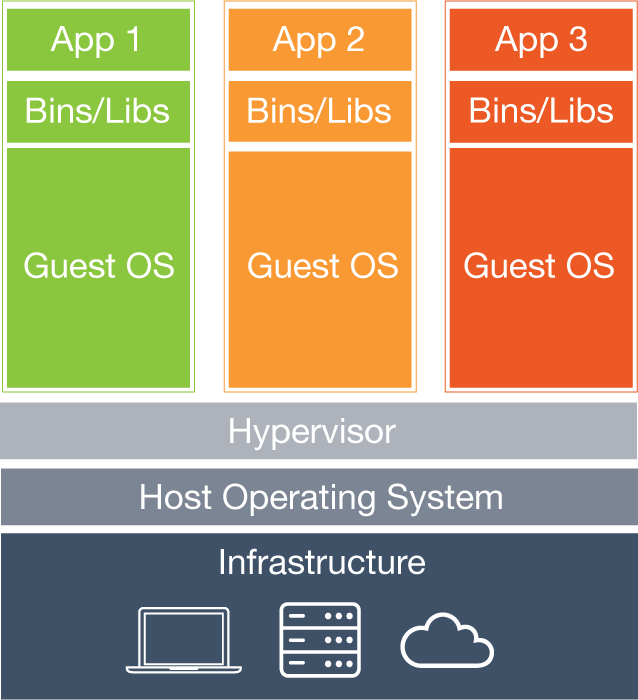
\includegraphics[width=\textwidth]{figs/docker-vm.png}
  \caption{Figure that shows how a normal virtual machine is built up.}
  \label{fig:vm-resources}
\end{subfigure}%

\begin{subfigure}{.5\textwidth}
  \centering
  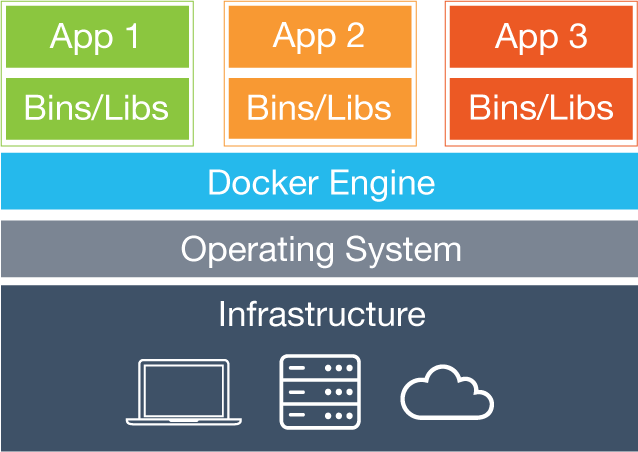
\includegraphics[width=\textwidth]{figs/docker-docker.png}
  \caption{Figure that shows  how a Docker container is built up.}
  \label{fig:docker-resources}
\end{subfigure}
\caption{Figures that shows the differences between a Docker container and a virtual machine. \cite{docker-what-is}}
\label{fig:docker-vm-resources}
\end{figure}


\subsubsection{Conclusion}
Based on experience and that new technology was wanted, the backend team went with a NodeJS-based backend solution. This lead to Express which was lightweight and had everything needed for building a RESTful API, and which a team member had experience with from before. Due to the unknown factors surrounding data structurization, and the fact that the team wanted JSON to be sent from the server, a document-oriented database system was chosen. The system that was chosen was MongoDB, which is the most used document-oriented database system, and well supported on the NodeJS-platform. It is well tested, and the necessary libraries are available. For data validation the team chose Joi due to customer recommendation. The tools Swagger and Postman helps to share, explore and test the API.


\subsection{Design}

\subsubsection{Mockup and design tools}
In order to plan and get feedback on the designs of the applications, it was necessary to create mockups. The mockups are presented to the customer, used as the basis for usability tests, and is a great way to create early prototypes for internal workshops. 

\begin{description}
    \item[Balsamiq] \hfill \\
        Balsamiq is a mockup and wireframing software for creating generic sketches of the initial design. It is used in the early stages of the project to explore design alternatives and to get feedback from the customer and potential users. The mockups has a rough feel by design, in order to point out that the design is not final or a suggestion for a final design. This shifts the focus from smaller details to the more fundamental design decisions of the application.\cite{balsamiq}
    \item[Omnigraffle] \hfill \\
        Omnigraffle is a digital illustration software and can be used for everything from initial sketches to detailed design. There are no included platform related elements, but there are libraries available for download if needed.\cite{omnigraffle} 
    \item[Proto.io] \hfill \\
        Proto.io is a website for creating detailed mockups with high precision. It supports platform specific elements, and was therefore used to create prototypes for Android.\cite{protoio}
\end{description}

Balsamiq was chosen to design the initial mockups. While Proto.io can be used for both iOS and Android sketches, the team decided to use Omnigraffle for iOS as the team has more experience with that tool. 
